\section{Representative Examples}
Given the theoretical framework for downfolding a many-orbital (or many electron) problem to a 
few orbital (or few electron) problem, we now discuss three examples which also serve to highlight some practical aspects 
associated with AIDMD. The first example is mostly pedagogical, 
where we have completely avoided the complications of low energy state generation, 
and the general difficulty of doing the ab-initio calculation itself. Rather, we use information directly available 
from \emph{exact} eigenstates themselves to downfold from a lattice model with more orbitals (three band model) 
to one with fewer orbitals (one band model). We then gradually increase the complexity of the problems we address
by downfolding the hydrogen chain in one dimension (with up to 10 atoms) and graphene 
(with up to 32 carbons on a 2D honeycomb lattice).
  
\subsection{Three-band Hubbard model to one band Hubbard model at half filling}
\subsubsection{Introduction}
%A big motivation for studying lattice models of strongly correlated systems comes from their 
%relevance to 
The high $T_c$ superconducting cuprates~\cite{Bednorz1986} are complex materials whose parent compounds 
are Mott insulators that display rich phase diagrams on electron or hole doping~\cite{Dagotto_RevModPhys, LeeWen_RevModPhys}. 
Many extensive works have been devoted to determining their model effective Hamiltonians and corresponding parameter 
values~\cite{Emery, ZhangRice, tJSpalek, Hybertsen_PRB1989, Hybertsen_PRB1990, Pavirini, Kent_Hubbard}. 

The low energy physics in the cuprates is primarily associated with the 2D planes of copper and oxygen (notated 
as the XY plane); this setup has been shown in Fig.~\ref{fig:threeband} for a $2 \times 2$ unit cell.
Accounting for the octahedral environment of copper ions, with support from electronic structure 
and quantum chemistry calculations~\cite{Dagotto_RevModPhys}, one infers 
that the five-fold \emph{d} orbital degeneracy of copper is lifted to make the 
highest singly filled orbital to be the one with $d_{x^2-y^2}$ character. 
The $p_x$ or $p_y$ oxygen orbitals (depending on their orientation relative to the copper) 
hybridize most strongly with $d_{x^2-y^2}$. Thus the minimal model for the cuprates involving the oxygens 
is the 3-orbital or 3-band Hubbard model, 
\BDB{What are sum over d? Should it be i, sigma?}
\begin{eqnarray}
H &=&    \epsilon_p \sum_{j,\sigma} n^{p}_{j,\sigma} + \epsilon_{d} \sum_{d}  n^{d}_{i,\sigma} 
	+ t_{pd} \sum_{\langle i,j \rangle, \sigma} \text{sgn}(p_i,d_j) \Big( d_{i,\sigma}^{\dagger} p_{j,\sigma} + \text{h.c.} \Big) \nonumber \\
  & &   + U_p \sum_{j} n^{p}_{j,\uparrow} n^{p}_{j,\downarrow} + U_d \sum_{i} n^{d}_{i,\uparrow} n^{d}_{i,\downarrow} + V_{pd} \sum_{\langle i,j \rangle} n^{j}_p n^{i}_d 
\end{eqnarray}
where $d_i,p_j$ refer to the orbitals of copper (at site $i$) and oxygen (at site $j$)  respectively 
and the signs of the hopping $t_{pd}$ between them are shown in Fig.~\ref{fig:threeband}. 
$\epsilon_p$,$\epsilon_d$ refer to the orbital energies, 
$U_d$, $U_p$ refer to strength of onsite Hubbard interactions and $V_{pd}$ refers to the 
stength of the density-density interactions between a neighboring $p$ and $d$ orbital. 
One could consider further variations of the model by adding $t_{pp}$ type hoppings, but 
these have not been shown here. To keep the exposition simple, we consider only 
the case where $\epsilon_p$, $t_{pd}$ and $U_{d}$ are non zero and 
since we work with a fixed number of particles, set $\epsilon_d = 0$. Thus the 
charge transfer energy $\Delta \equiv \epsilon_p - \epsilon_d$ equals $\epsilon_p$ in our notation. 
We find it convenient to work in the hole notation and thus half filling corresponds to 2$\uparrow$ and 2$\downarrow$ 
holes on the $2\times2$ cell.

\begin{figure}[htpb]
\centering
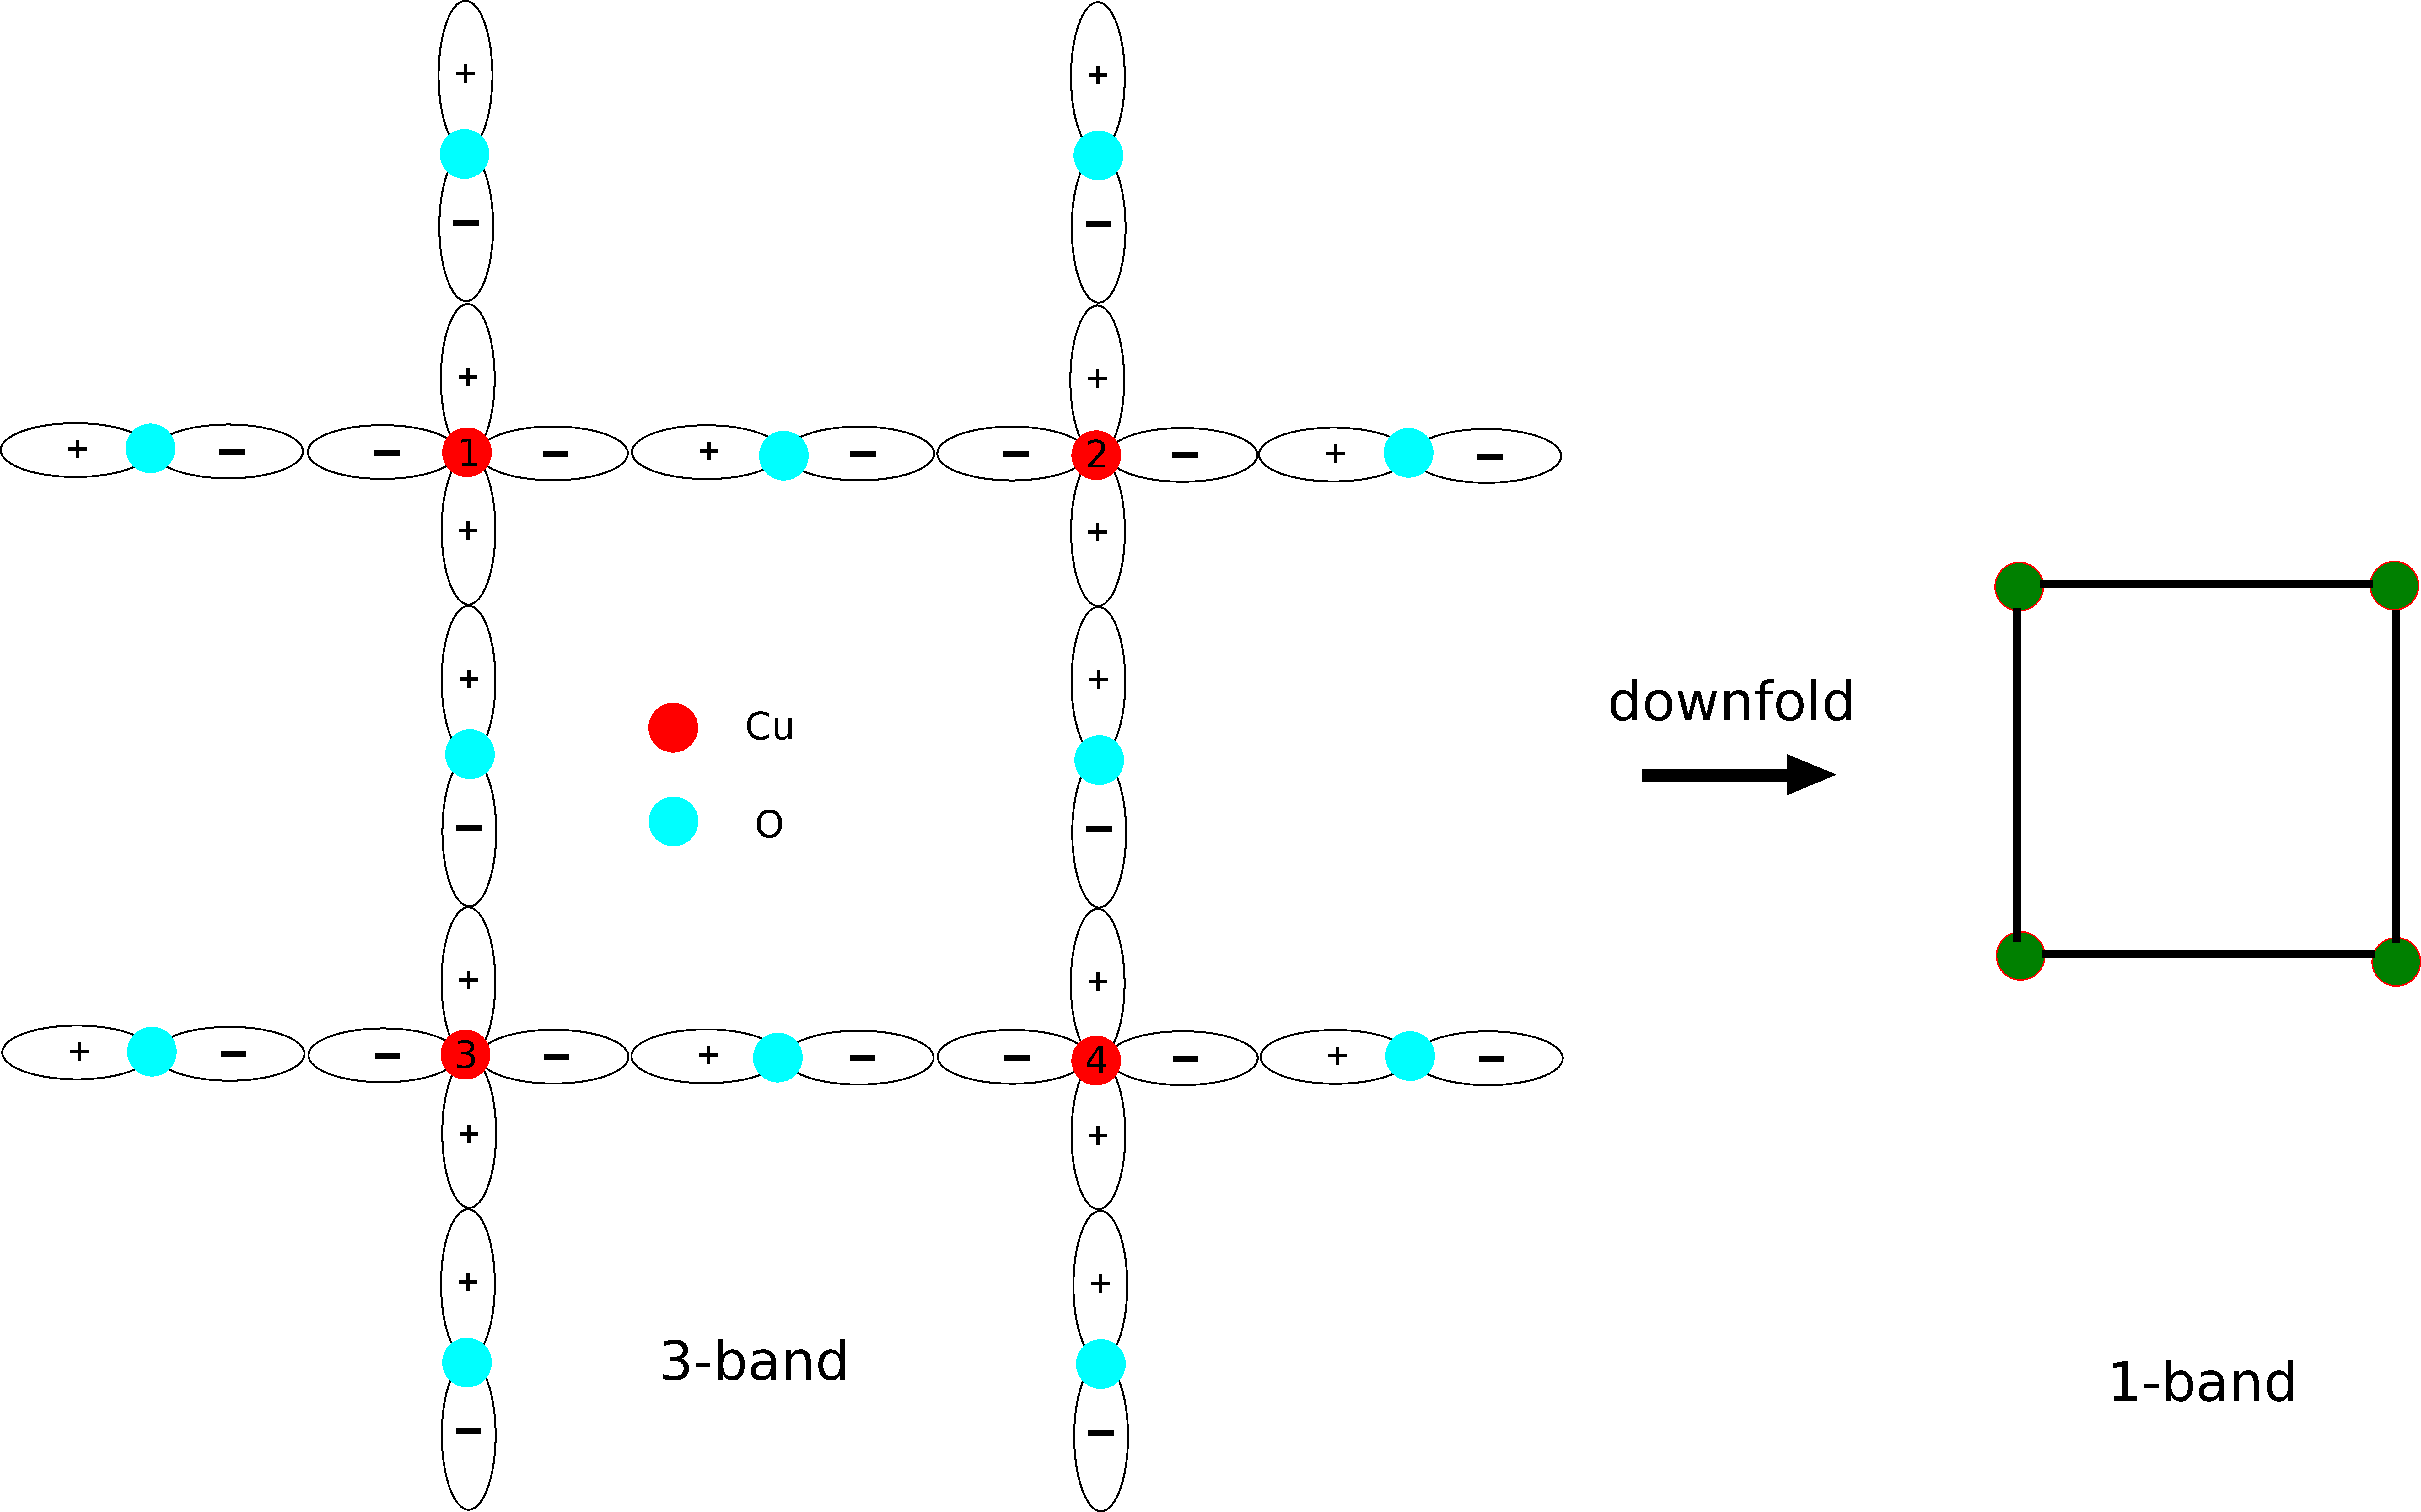
\includegraphics[width=1\linewidth]{./Figures/three_band_figure.pdf}
\caption{Schematic for downfolding the three band Hubbard model to the one band Hubbard model. 
The oxygen orbitals are completely eliminated to give "dressed" $d$-like orbitals of the one band model, with modified hopping 
and interaction parameters.}
\label{fig:threeband} 
\end{figure}	

The justification for the 3-band model for the cuprates, along with the determination of its parameters, 
is itself contingent on downfolding from an \emph{ab-initio} calculation, 
of the type carried out in Refs.~\cite{Wagner_Abbamonte}. (There is also suggestion that the 4s orbital of copper is important 
for the low energy properties~\cite{Pavirini} but we steer clear of these debates here.) 
Instead we use the 3-band model at half filling, as a prototypical example of what it \emph{means} to downfold to 
a simpler model - the one band Hubbard model, 
\begin{eqnarray}
	\tilde{H} &=&  -t \;\sum_{\langle i,j \rangle} \tilde{d}_i^{\dagger} \tilde{d}_j + U \;\sum_{i} \tilde{n}^{i}_{\uparrow} \tilde{n}^{i}_{\downarrow}
\label{eq:oneband}
\end{eqnarray}
where $t$ and $U$ are downfolded (renormalized) Hubbard parameters, which are to 
be determined for given 3-band parameters, and $\tilde{d}$ are the effective \emph{d-like} orbitals. 
The latter are a mixture of copper and oxygen orbitals and this optimal transformation also remains an unknown. Thus, 
the determination of effective Hamiltonians is a \emph{dual} problem - (1) what are the composite objects that give a 
compact description of the low energy physics? and given this choice what are the effective interactions between them?  
This example will serve as a setting for the downfolding of more complex \emph{ab-initio} systems to lattice 
models. 

\subsubsection{Choice of effective one particle basis}
To map the three-band model to the one-band model and determine its validity, 
our first aim will be to obtain effective "dressed" \emph{d-like} 
orbitals that enter Eq.~\ref{eq:oneband}. We encode this relationship as 
the transformation ${\bf T}$, 
\begin{equation}
	\tilde{d}_i = \sum_{j} T_{ij} c_j
\end{equation}
where $\tilde{d}_i$ is a transformed hole (destruction) operator and $c_j$ is the bare hole (destruction)
operator, the latter could refer to either the bare $d$ or $p$ orbitals. Accounting for all symmetries of 
the $2\times2$ unit cell, {\bf T} is a $4 \times 12 $ matrix (the numbering of the orbitals 
corresponds to Fig.~\ref{fig:threeband}) is explicitly written out as, 
\begin{eqnarray}
{\bf T} = 
\left(
\begin{array}{cccccccccccc}
F        & \alpha_2 &        \alpha_2 &  \alpha_4 & \alpha_1 & \alpha_1 & -\alpha_1 & -\alpha_1 & \alpha_3 & -\alpha_3 & \alpha_3 & -\alpha_3 \\
\alpha_2 &  F       &        \alpha_4 &  \alpha_2 & \alpha_3 & -\alpha_1 & \alpha_1 & -\alpha_3 & -\alpha_3 & \alpha_3 & \alpha_1 & -\alpha_1 \\
\alpha_2 & \alpha_4 & F               &  \alpha_2 & -\alpha_1 & \alpha_3 & -\alpha_3 & \alpha_1 & \alpha_1 & -\alpha_1 & -\alpha_3 & \alpha_3 \\
\alpha_4 & \alpha_2 & \alpha_2        &   F       & -\alpha_3 & -\alpha_3 & \alpha_3 & \alpha_3 & -\alpha_1 & \alpha_1 & -\alpha_1 & \alpha_1 \\
\end{array}
\right)
\end{eqnarray}
where we have defined $F \equiv \sqrt{1-4{\alpha_1}^2 - 2{\alpha_2}^2 - 4 {\alpha_3}^2 -{\alpha_4}^2}$ and 
where the parameters $\alpha_1$,$\alpha_2$,$\alpha_3$ and $\alpha_4$ will be 
optimized to minimize a certain cost function, which will be explained shortly. 

Note that the transformation has been chosen to be a linear one. One can imagine a more complicated 
many-body transformation involving higher body functions. In practice, at least for the model under 
consideration, this does not seem to be necessary. 
%This does not mean that determining the optimal one body space is \emph{always} a trivial problem. 
%In fact, (as pointed out to us by D. Ceperley) there are several interesting problems in the study of helium 
%that involve ring exchanges involving as many as 12 particles~\cite{Ceperley_Jacucci}, 
%certainly our simple minded transformation does not capture the search for such multi-body 
%or composite objects. However, for the purpose of the rest of the paper, we will show the utility 
%of the linear transformations even for the \emph{ab-initio} to lattice downfolding cases; 
%Kohn Sham orbitals will be rotated to form localized functions. These one body transformations will give us the orbitals 
%that enter the definition of the effective Hamiltonian. 

The one particle density matrix in the transformed basis is related 
to that in the original basis by,
\begin{equation}
	\langle {\tilde{d}_i}^{\dagger} \tilde{d}_{j} \rangle = \sum_{mn} T^{*}_{im} \langle {c_m}^{\dagger} c_n \rangle T_{jn}
\end{equation}
and using this relationship we demand two conditions be satisfied,
\begin{itemize} 
 \item The effective orbitals are orthogonal to each other 
 \item All diagonal entries of the 1-RDM of the effective orbitals for all low energy eigenstates 
       $(\langle {\tilde{d}_i}^{\dagger} \tilde{d}_{i} \rangle)$ 
       equal 1/2.
\end{itemize} 
We consider a cost function, 

\subsubsection{Results and Discussion}
To give a concrete and representative example of our results, we start with 1-RDM of the lowest eigenstate 
in either $\uparrow$ or $\downarrow$ channel. This is a $12 \times 12$ matrix, which for $U_{d}/t_{pd}=8$ 
and $\Delta/t_{pd}=3$ we find to be,
\begin{eqnarray}
\left(
\begin{array}{cccccccccccc}
+0.380	   & -0.091 &-0.091 &-0.015& +0.119& +0.119& -0.119 &-0.119 &-0.017 &+0.017 &-0.017 &+0.017 \\
-0.091	   & +0.380 &-0.015 &-0.091& -0.017& -0.119& +0.119 &+0.017 &+0.017 &-0.017 &+0.119 &-0.119 \\
-0.091	   & -0.015 &+0.380 &-0.091& -0.119& -0.017& +0.017 &+0.119 &+0.119 &-0.119 &+0.017 &-0.017 \\
-0.015	   & -0.091 &-0.091 &+0.380& +0.017& +0.017& -0.017 &-0.017 &-0.119 &+0.119 &-0.119 &+0.119 \\
+0.119	   & -0.017 &-0.119 &+0.017& +0.060& +0.034& -0.034 &-0.060 &-0.034 &+0.034 &-0.007 &+0.007 \\
+0.119	   & -0.119 &-0.017 &+0.017& +0.034& +0.060& -0.060 &-0.034 &-0.007 &+0.007 &-0.034 &+0.034 \\
-0.119	   & +0.119 &+0.017 &-0.017& -0.034& -0.060& +0.060 &+0.034 &+0.007 &-0.007 &+0.034 &-0.034 \\
-0.119	   & +0.017 &+0.119 &-0.017& -0.060& -0.034& +0.034 &+0.060 &+0.034 &-0.034 &+0.007 &-0.007 \\
-0.017	   & +0.017 &+0.119 &-0.119& -0.034& -0.007& +0.007 &+0.034 &+0.060 &-0.060 &+0.034 &-0.034 \\
+0.017	   & -0.017 &-0.119 &+0.119& +0.034& +0.007& -0.007 &-0.034 &-0.060 &+0.060 &-0.034 &+0.034 \\
-0.017	   & +0.119 &+0.017 &-0.119& -0.007& -0.034& +0.034 &+0.007 &+0.034 &-0.034 &+0.060 &-0.060 \\
+0.017	   & -0.119 &-0.017 &+0.119& +0.007& +0.034& -0.034 &-0.007 &-0.034 &+0.034 &-0.060 &+0.060 \\
\end{array}
\right)
\end{eqnarray}
and transform it into a $4\times4$ RDM (satisfying the requirements of our cost function), 
\begin{eqnarray}
\left(
\begin{array}{cccc}
+0.499 & -0.158 & -0.158 & 0.000  \\
-0.158 & +0.499 &  0.000 & -0.158 \\
-0.158 &  0.000 & +0.499 & -0.158 \\
 0.000 & -0.158 & -0.158 & +0.499 \\
\end{array}
\right)
\end{eqnarray}
corresponding to the optimal parameters $\alpha_1=0.220$,$\alpha_2=0.044$,$\alpha_3=0.020$ and $\alpha_4=0.018$ 
We then ask what $U/t$ of the one band Hubbard model best describes this 1-RDM and in this case find $U/t = $. 
Similar results are found when one considers the other low energy eigenstates. 
(In practice, we minimize the sum of costs of the lowest three eigenstates on the $2 \times 2$ cluster.) 

\begin{figure}[]
\centering
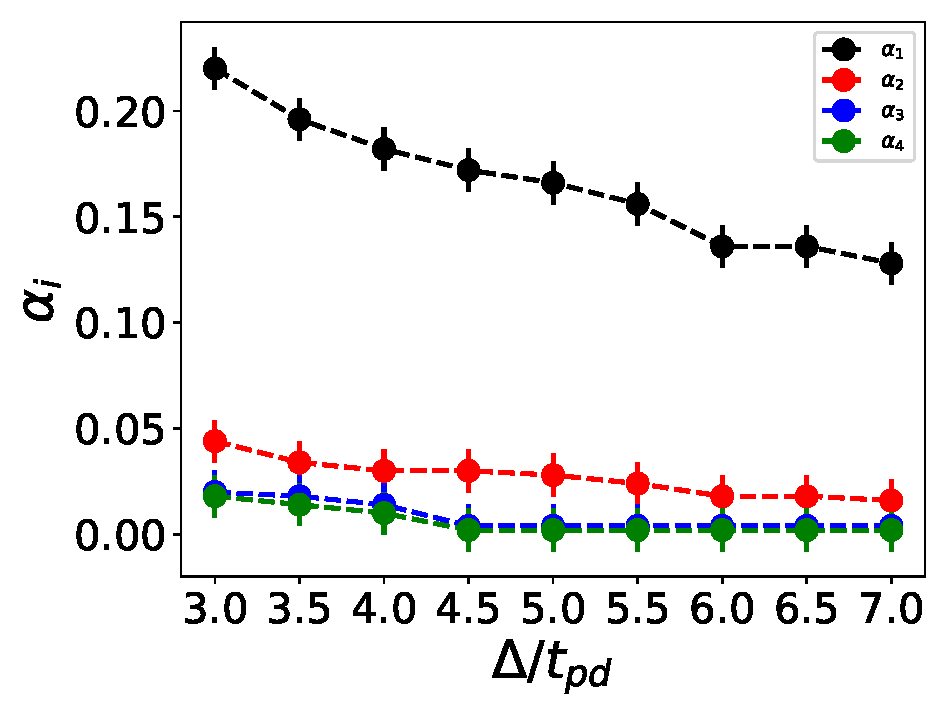
\includegraphics[width=0.49\linewidth]{./Figures/Hyb_vs_U_Ud_8.pdf}
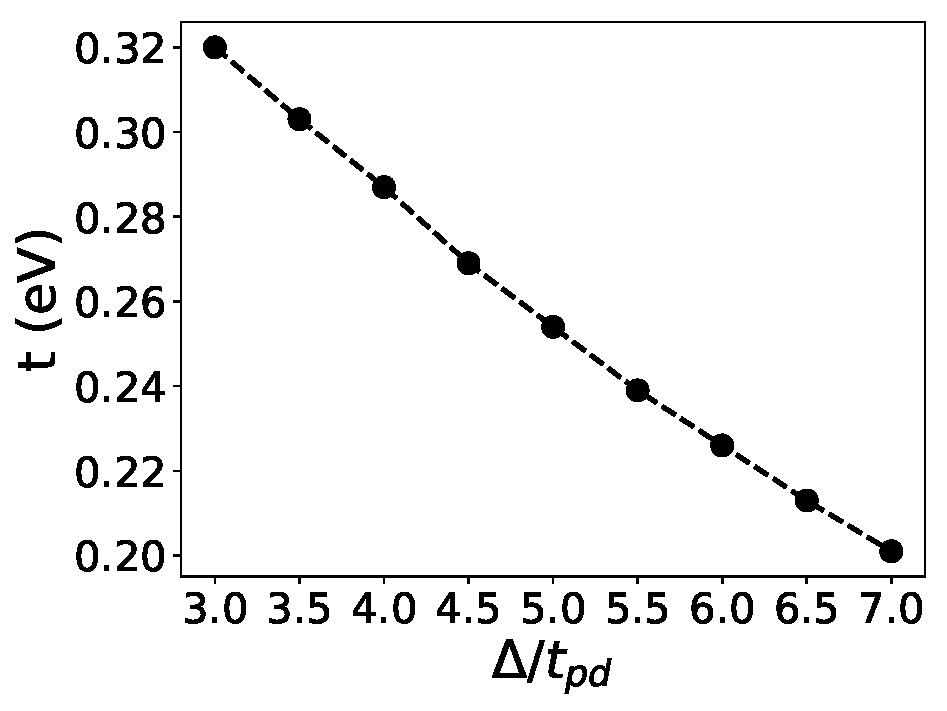
\includegraphics[width=0.49\linewidth]{./Figures/Hopping_vs_U_Ud_8.pdf}
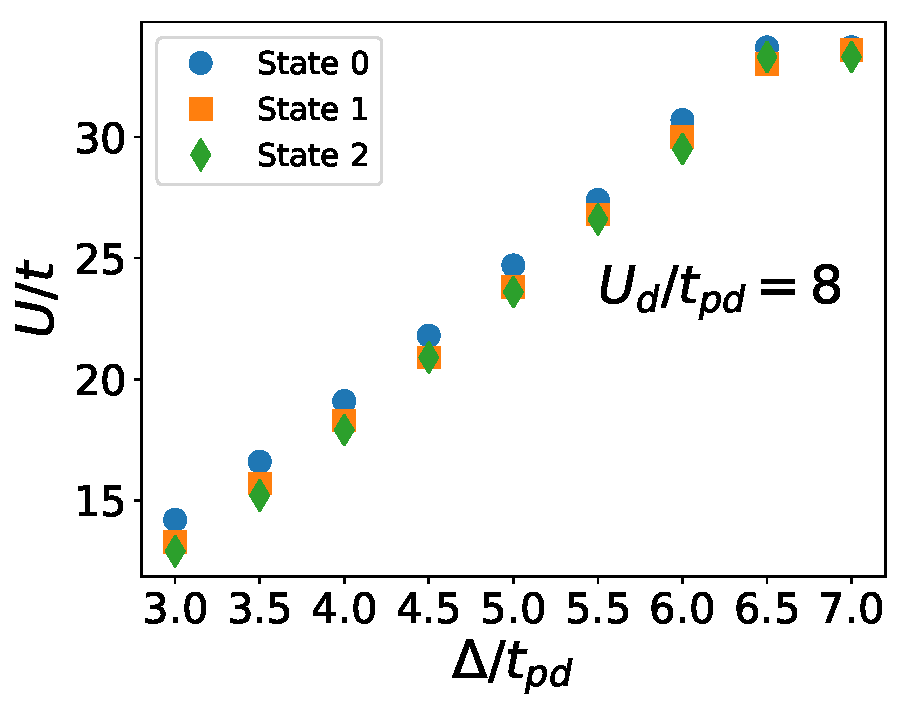
\includegraphics[width=0.49\linewidth]{./Figures/downfolded_U_Ud_8.pdf}
\caption{Downfolded values of the effective 1-band Hubbard U/t and hopping $t_{opt}$ vs $U_d/t_{pd}$}
\label{fig:hamfit} 
\end{figure}	

\begin{figure}[]
\centering
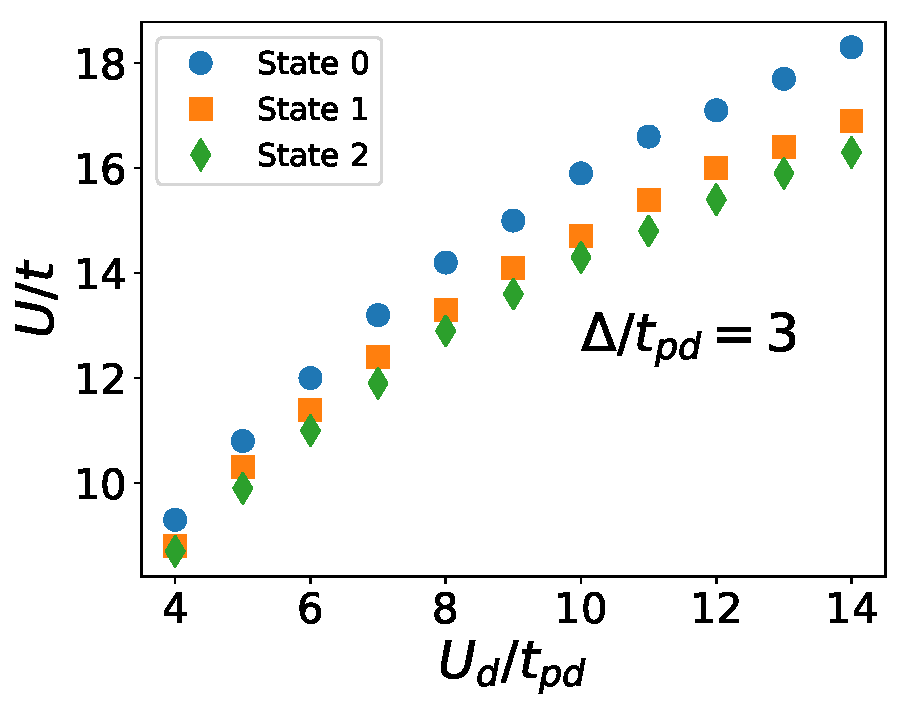
\includegraphics[width=0.49\linewidth]{./Figures/downfolded_U_ep_3.pdf}
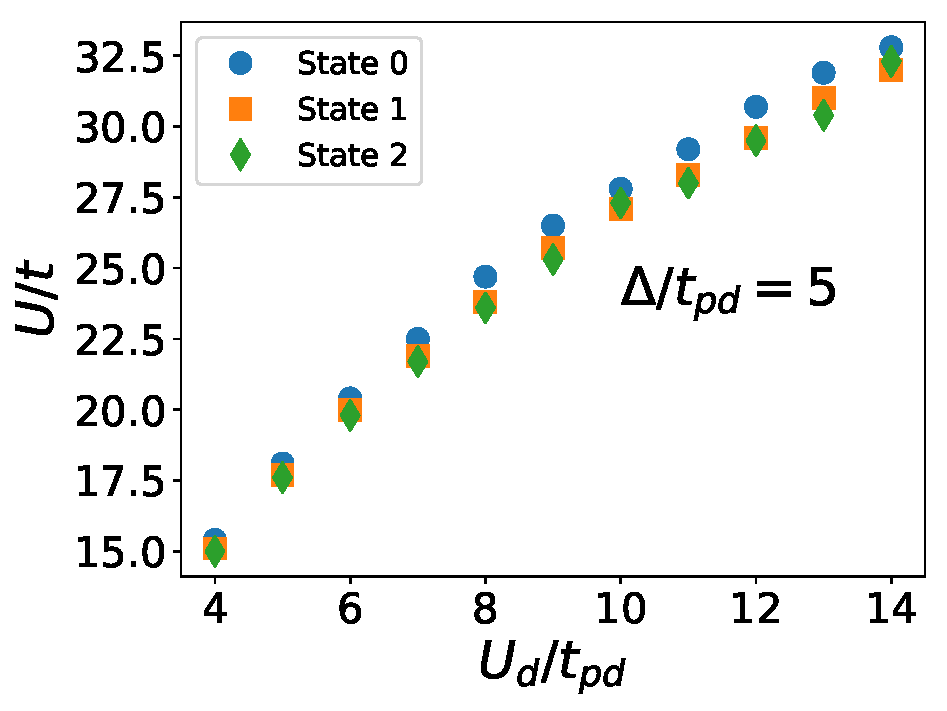
\includegraphics[width=0.49\linewidth]{./Figures/downfolded_U_ep_5.pdf}
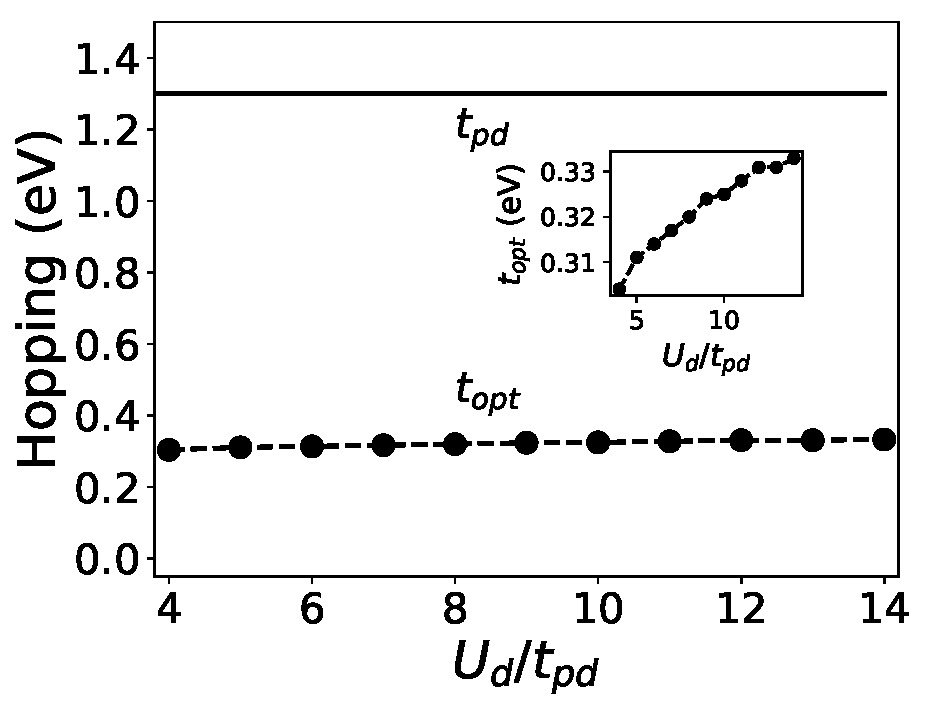
\includegraphics[width=0.49\linewidth]{./Figures/Hopping_vs_U_ep_3.pdf}
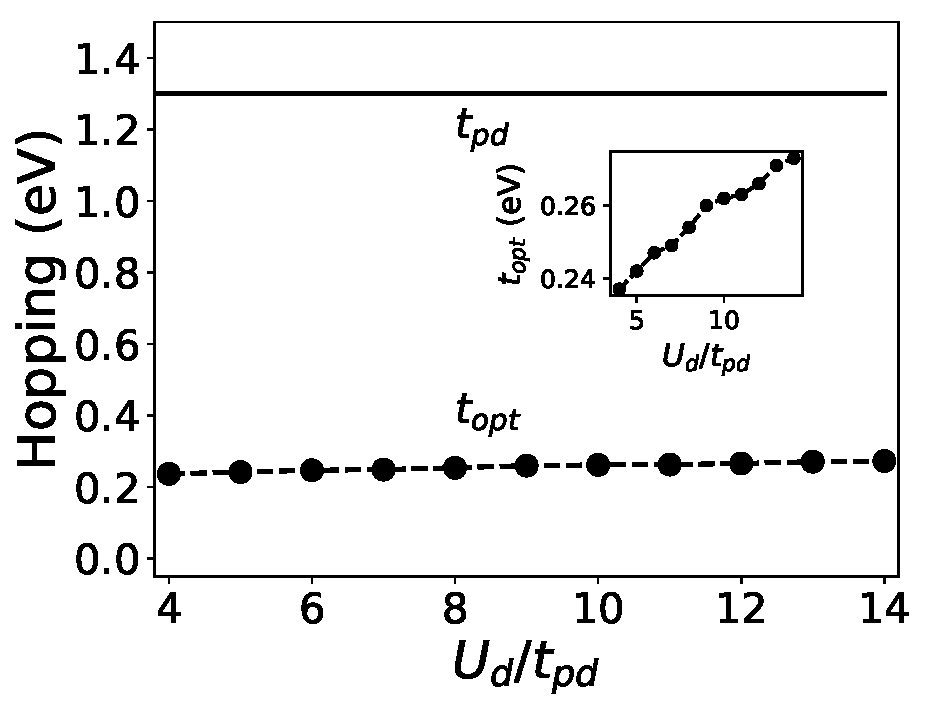
\includegraphics[width=0.49\linewidth]{./Figures/Hopping_vs_U_ep_5.pdf}
\caption{Downfolded values of the effective 1-band Hubbard U/t and hopping $t_{opt}$ vs $U_d/t_{pd}$}
\label{fig:hamfit} 
\end{figure}	
 
The density matrix matching does not provide an absolute energy scale for the matching. 
Taking $t_{pd}$ to be the typical values of $1.3$ eV, we then 
We show our results for the optimal values of $t$ and the transformation parameters for different $\Delta/t_{pd}$
keeping $U_d/t_{pd}=8$ fixed. First, note that $\alpha_1$, which is the primary parameter that mixes (hybridizes) 
the copper and oxygen orbitals, \emph{decreases} as $\Delta/t_{pd}$ is increased. This is physically reasonable 
since an increasing difference in the single particle energies of the copper and oxygen orbitals 
means that it is even more energetically unfavorable to occupy the oxygen orbitals. 
Correspondingly the effective hopping between $\tilde{d}$ in the 
1-band model reduces and the effective $U/t$ increases. 

Next, we consider our results for  

These results are only useful if the energy spectra between the two models also matches. This is verified 
and demonstrated for some representative examples in Fig.        

\begin{figure}[]
\centering
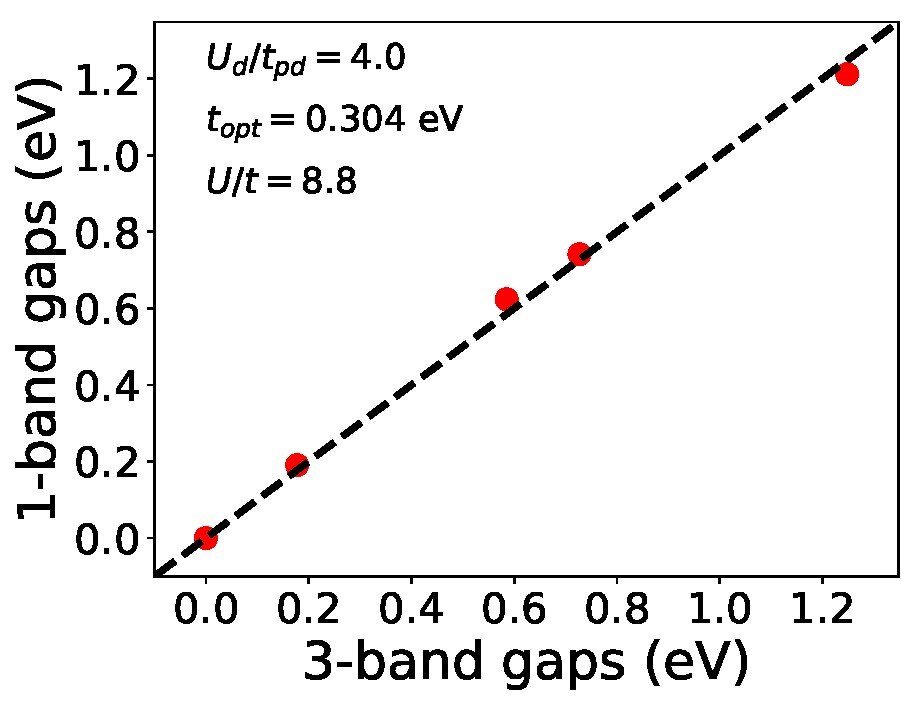
\includegraphics[width=0.325\linewidth]{./Figures/Gap_1_band_3_band_ep_3_number_5.pdf}
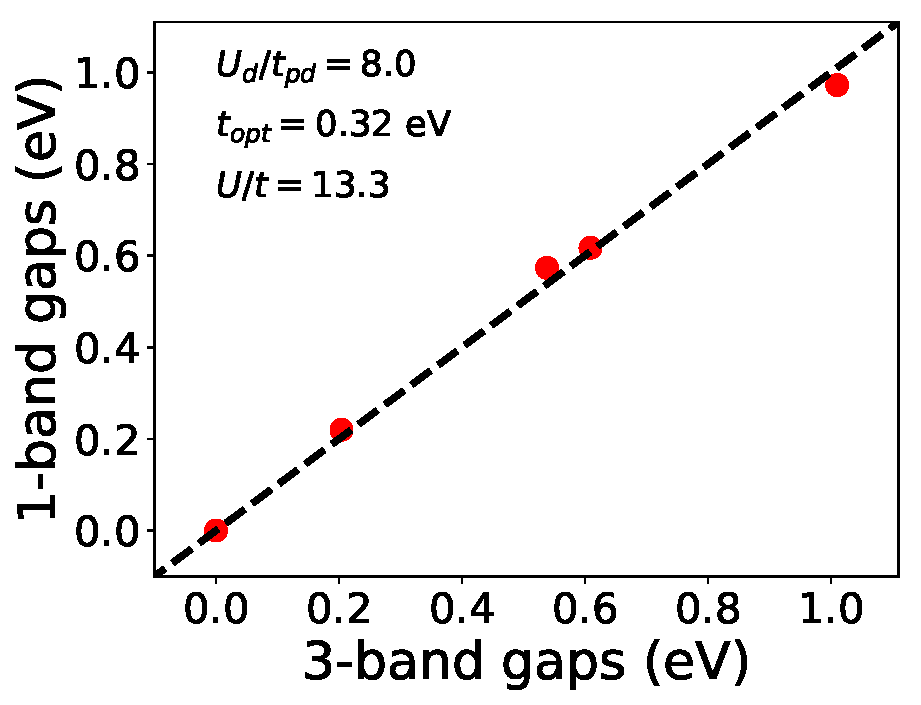
\includegraphics[width=0.325\linewidth]{./Figures/Gap_1_band_3_band_ep_3_number_9.pdf}
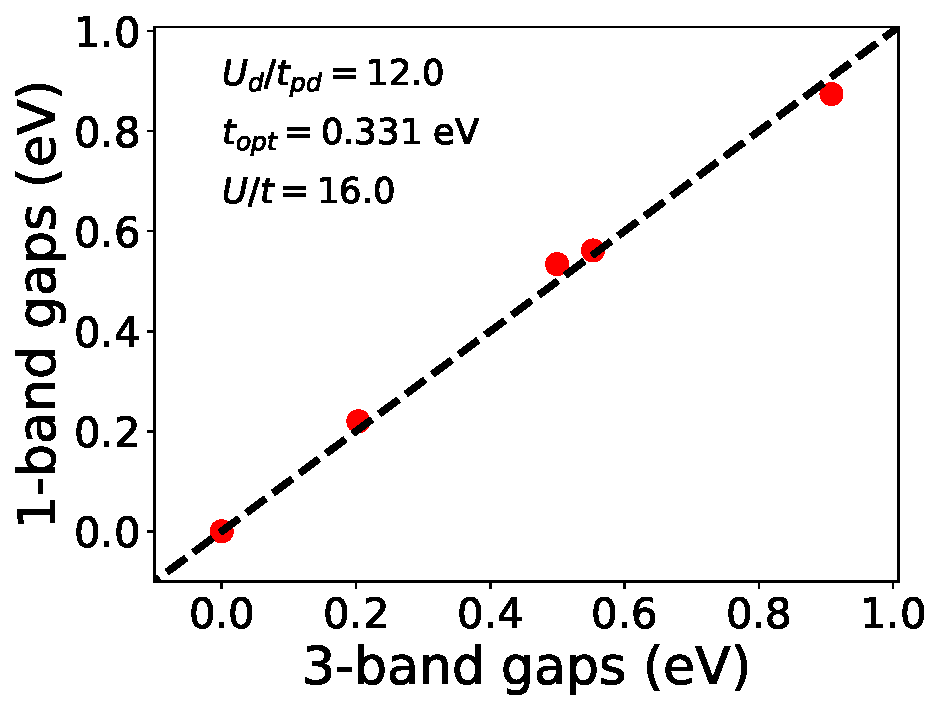
\includegraphics[width=0.325\linewidth]{./Figures/Gap_1_band_3_band_ep_3_number_2.pdf}
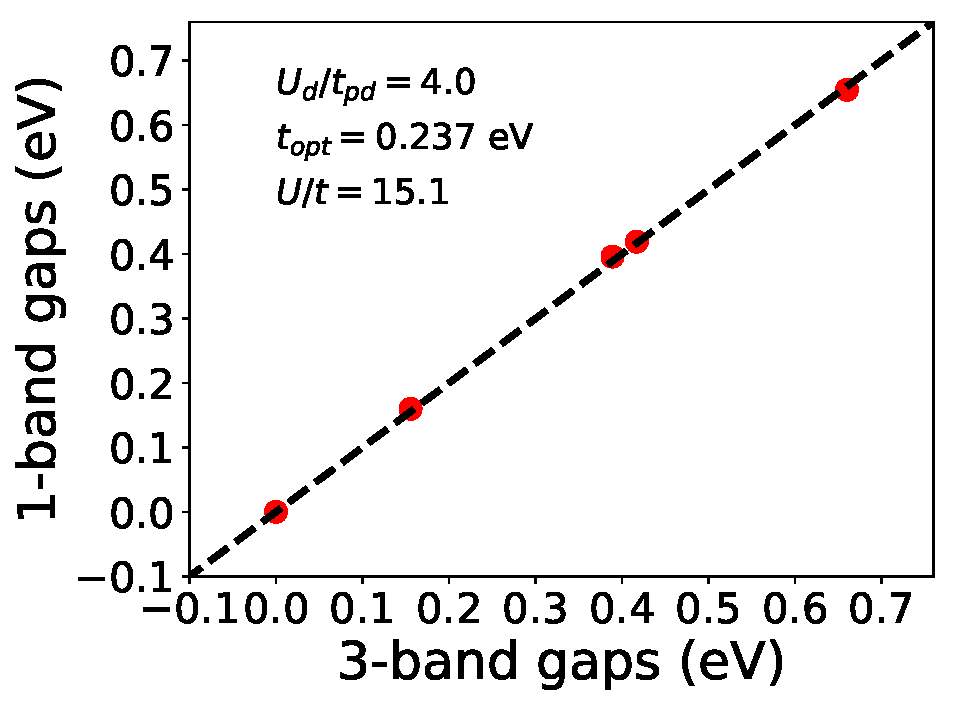
\includegraphics[width=0.325\linewidth]{./Figures/Gap_1_band_3_band_ep_5_number_5.pdf}
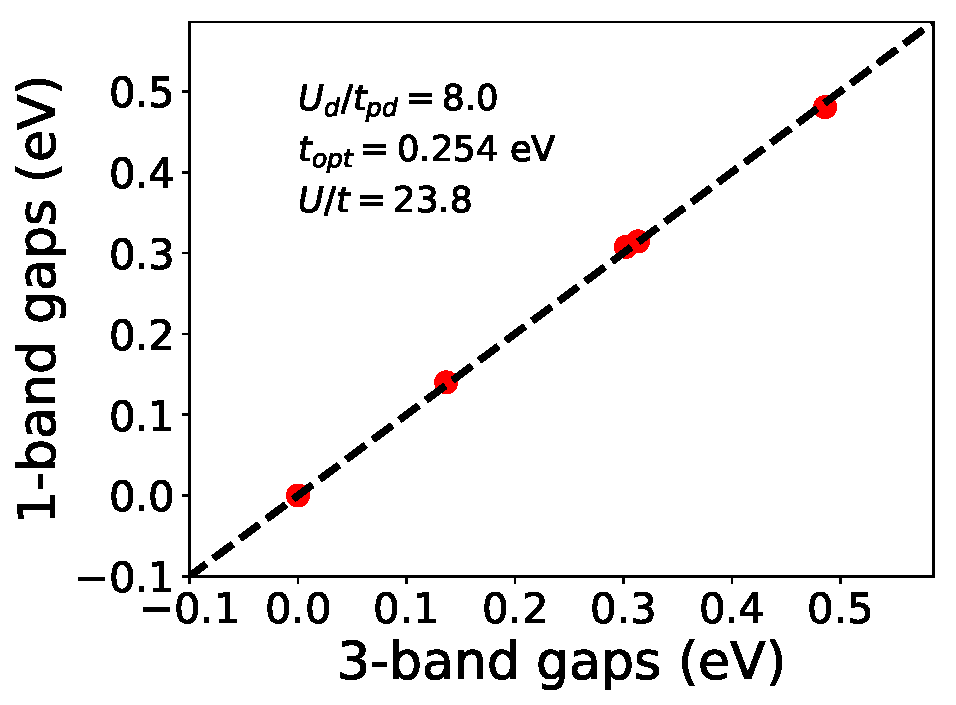
\includegraphics[width=0.325\linewidth]{./Figures/Gap_1_band_3_band_ep_5_number_9.pdf}
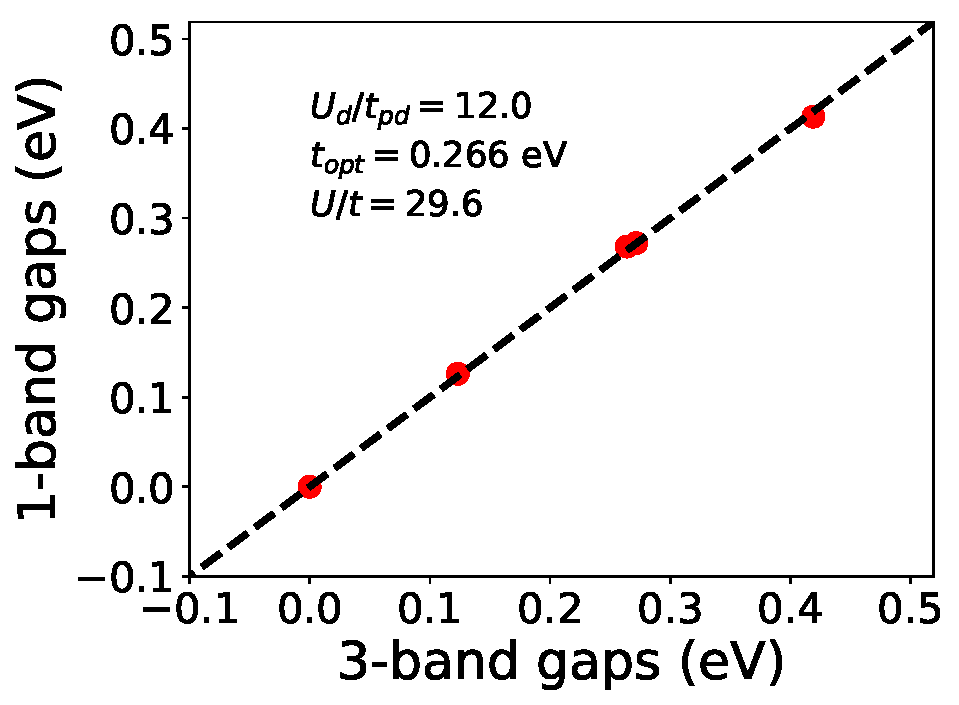
\includegraphics[width=0.325\linewidth]{./Figures/Gap_1_band_3_band_ep_5_number_2.pdf}
\caption{Comparison for energy gaps between the 3-band and 1-band Hubbard models using the optimized values of $U/t$ and $t$, for different
$U_{d}/t_{pd}$ for $\Delta/t_{pd}=3$ and $\Delta/t_{pd}=5$}
\label{fig:hamfit} 
\end{figure}	

 
Finally, we show that the obtained parameters are ....


